\chapter{Modelling Review}
\begin{nolinkcolors} 
\minitoc
\end{nolinkcolors}
\newpage

%***********************************************
\section{Modelling macrosegreation}
%***********************************************
%
%***********************************************
\subsubsection{Microsegregation models}
%***********************************************
Solid formation depends greatly on the ability of chemicals species to diffuse within each of 
the solid and liquid phases, %but also across the solid-liquid interface. 
Furthermore, chemical diffusion like all other 
diffusional processes, is a time-dependent phenomenon. One can thus conclude that two factors
influence the amount of solid formation: cooling rate and diffusion coefficients. However, 
convection and other mechanical mixing sources, homogenise the composition much faster than atomic diffusion. 

Considering that $D^l/D^s\approx$\num{d3}-\num{d4} for species within the solidification interval, \emph{complete mixing} in the liquid is often an acceptable assumption, regardless of the 
solidification time. Thus, we speak of infinite diffusion in the liquid. Diffusion in the solid, 
also known as \emph{back diffusion}, is the only transport mechanism with very low diffusion coefficients. 
Therefore, chemical species require a long time, i.e. low cooling rate, to completely diffuse within the solid.
The difference in diffusional behaviour at the scale of a secondary dendrite arm, is summarised by two limiting 
segregation models of perfect equilibrium  and non-equilibrium, which are the lever rule and Gulliver-Scheil models, respectively. 
Afterwards, models with finite back diffusion are presented. 
%------------

%***********************************************
\subsubsection*{Lever rule}
%***********************************************

The lever rule approximation considers ideal equilibrium in and between all phases. It requires a long solidification time, i.e. extremely slow cooling rate, hence phase compositions are 
homogeneous ($ \Clstar = \Cl$ and $ \Csstar = \Cs$ ) at all times as a consequence of complete mixing. 
These compositions are given by:
%----------------------
\begin{align}
\label{eq:leverrule}
& \Cl= \Clstar = \k^{-1} \Csstar = \k^{-1} \Cs \\
& \Cs= \Csstar = \frac{\k \Cnominal}{\k\fs + (1-\fs)}
\end{align}
%----------------------
where $\Cl$ and $\Cs$ are the phase compositions and $\Clstar$ and $\Csstar$ are values at the solid-liquid interface in 
the liquid and solid phases, respectively.  At the end of solidification, if a single solid phase forms, its composition is equal to the nominal composition, $\Cs = \Cnominal$.
%------------

%***********************************************
\subsubsection*{Gulliver-Scheil}
%***********************************************

The other limiting case is the absence of diffusion in the solid or its limitation due to fast cooling.
For a segregation coefficient less than unity, the consequence is a steady increase  of the homogeneous liquid composition
upon cooling while the solid composition continuously increases and becomes non-uniform.
Compared to a full equilibrium approach, higher fractions of liquid will remain. In eutectic systems, liquid may exist until 
another solid structure forms, e.g. upon reaching the eutectic composition, 
triggering a eutectic solidification, that is the appearance of the lamellar eutectic microstructure. 
Assuming phase equilibrium is still valid, i.e. $\Clstar=\k^{-1} \Csstar$, the phase compositions are given by:
%----------------------
\begin{align}
\label{eq:scheil1}
& \Cl= \Clstar = \k^{-1} \Csstar \\
\label{eq:scheil2}
& \Csstar= \k \Cnominal (1-\fs)^{\k-1} \\
\label{eq:scheil3}
& \Cs = \int_{0}^{f^s} \Csstar\: \mathrm{d}f^s
\end{align}
%------------
%***********************************************
\subsubsection*{Finite back diffusion}
%***********************************************
The assumption of a negligible back diffusion overestimates the liquid composition
and the resulting eutectic fraction. Therefore, many models studied the effect of limited diffusion in the solid. 
One of the earliest models is the Brody-Flemings models \citep{brody_solute_1966} that is a based on a differential solute balance equation for a parabolic growth rate, as follows:
%khan_influence_2014
%----------------------
\begin{align}
\label{eq:brodyflemings}
& \Cl= \Clstar = \k^{-1}  \Csstar \\
& \Csstar= \k \Cnominal \crochet{ 1 - \brac{ 1 - 2 \Fos \k } \fs }^{\frac{\k-1}{1 - 2 \Fos \k }}
\end{align}
%------------
where $\Fos$ is the dimensionless \emph{Fourier number} for diffusion in the solid \citep{dantzig_solidification_2009}. 
It can be defined using the solid diffusion coefficient $\Ds$, solidification time $\tsolidif$ and the secondary 
dendrite arm spacing, $\sdas$, as follows: 
%----------------------
\begin{align}
\label{eq:fouriersolid}
& \Fos = \frac{D^s \tsolidif}{\brac{\sdas / 2}^2}
\end{align}
%------------
Several other models were since suggested and used. The interested reader is referred to the following non 
exhaustive list of publications: \citet{clyne_solute_1981,kobayashi_solute_1988,ni_volume-averaged_1991,wang_multiphase_1993,
combeau_modeling_1996,martorano_solutal_2003,tourret_generalized_2009}. It is noted that some of these publications consider 
also a finite diffusion in the liquid phase. It also noted that dealing with some aspects 
(e.g. multicomponent equilibrium phase diagrams, cross-diffusion of species, ...) is generally difficult
and received a limited number of studies in the aim of determining a multicomponent segregation model, thus numerical approaches are favoured.
%------------------------------------

%***********************************************
\subsection{Macroscopic solidification model: monodomain} \label{sec:monodomain}
%***********************************************
In this section, we will present the macroscopic conservations equations that enable us to predict 
macrosegregation in single multiphase metal system.
%***********************************************
\subsubsection{Volume averaging} \label{sec:volumeavg}
%***********************************************
It is crucial for a solidification model to represent phenomena on the microscale, then scale up to predict 
macroscopic phenomena. Nevertheless, the characteristic length of a small scale in solidification may be represented by a dendrite arm spacing, 
for instance for the mushy zone permeability, as it may also be represented by an atomic distance if one is interested, 
for instance in the growth competition between diffusion and surface energy of the solid-liquid interface.
Modelling infinitely small-scale phenomena could be prohibitively expensive in computation time, if we target industrial scales.
Therefore, the common volume averaging approach alleviates these difficulties by making assumptions on intermediate scales. 
This technique allows bypassing this barrier by averaging small-scale variations on a so-called 
\emph{representative volume element} (RVE) \citep{dantzig_solidification_2009} of volume \rev, with the following 
dimensional constraints: the element should be large enough to "see" and average microscopic fluctuations 
whilst being smaller than the scale of macroscopic variations.

Solid and liquid may exist simultaneously in the RVE, but we may also consider that no gas phase could be 
added (i.e. volume saturation with $\Vs+\Vl=\rev$). Moreover, temperature is generally assumed uniform and equal for all the phases.
The formalism, introduced by \citet{ni_volume-averaged_1991}, introduces a phase indicator function
for any phase $\phi$ in the multiphase system:
% ----------------------
\begin{align}
\label{eq:phase_indicator}
% \chi^\phi(x,t)=
\chi^\phi=
\begin{cases}
  1 	& \text{in } \phi \\ 
  0 	& \text{otherwise}
\end{cases}
\end{align}
% ----------------------
Then the approach suggests the following equations for any physical quantity $\psi$ in system containing
solid ($s$) and liquid ($l$) phases:
%----------------------
\begin{align}
\label{eq:volumeaveraging1}
& \avg{\psi} = \frac{1}{\rev} \integral{\rev}{\psi}{\Omega} = \avg{\psi^s} + \avg{\psi^l}
\end{align}
%------------
where $\psis$ and $\psil$ are phase averages of $\psi$. Then, for any phase $\phi$, one can introduce the \emph{phase intrinsic average} of $\psi$, denoted $\avg{\psi}^\phi$, by writing:
%----------------------
\begin{subequations}
\begin{align}
\label{eq:volumeaveraging2}
 \avg{\psi^\phi} = \avg{\chi^\phi \psi} 
				&=\frac{1}{\rev} \integral{\rev}{\chi^\phi \psi}{\Omega} \\
\label{eq:volumeaveraging2b}
				&=\frac{1}{\rev} \integral{\Vphi}{\chi^\phi \psi}{\Omega} \\ 
\label{eq:volumeaveraging2c}
				&=\frac{\Vphi}{\rev} \brac{\frac{1}{\Vphi} \integral{\Vphi}{\chi^\phi \psi}{\Omega}} \\ 
\label{eq:volumeaveraging2d}
				&= \gphi \avg{\psi}^\phi
\end{align}
\end{subequations}
%------------
where $\gphi$ is the volume fraction of phase $\phi$ with $\gphi=V_\phi/\rev$. 
The transition from \cref{eq:volumeaveraging2} to \cref{eq:volumeaveraging2b} is the consequence of \cref{eq:phase_indicator}.
To finalize, the averaging is applied to temporal and spatial derivation operators:
%\citep{rivaux_simulation_2011}:
\begin{align}
\label{eq:volumeaveraging3}
& \avg{ \frac{\partial \psi}{\partial t} ^\phi } = \frac{\partial \avg{\psi^\phi}}{\partial t} - \integral{\Gamma_{\liqsol}}{\psi^\phi \vstar \cdot \vec{n^\phi}}{A} \\
\label{eq:volumeaveraging4}
& \avg{ \nabvec \cdot \vec{\psi^\phi} } = \nabvec \cdot \avg{\vec{\psi^\phi}} + \integral{\Gamma_{\liqsol}}{\vec{\psi^\phi} \cdot \vec{n^\phi}}{A}
\end{align}
%------------

where $\vstar$ is the local relative interface velocity and $\Gamma_{\liqsol}$ is the solid-liquid interface, 
while $n^\phi$ is the normal to $\Gamma_{\liqsol}$, directed outwards. The surface integral terms in 
\cref{eq:volumeaveraging3,eq:volumeaveraging4} are \emph{interfacial averages} 
that express exchanges between the phases across the interface. The previous equations will 
be used to derive a set of macroscopic conservation equations. 
% It is noted that the intrinsic average $\avg{\psi}^\phi$ may be replaced by ${\psi}^\phi$ 
% for notation simplicity, whenever the averaging technique applies.
% This notation is thus compatible with the previously introduced average defined for the solid composition when the latter is non-uniform \cref{eq:scheil3}.

%***********************************************
\subsubsection{Macroscopic equations}
%***********************************************

A monodomain macroscopic model relies on four main conservation equations to predict 
macrosegregation in a single alloy where the latter is considered without any direct representation of interactions with another
domain (moulds, air, ...). 
The general form of such a macroscopic conservation equation is given by:

%-----------
\begin{align}
\label{eq:conservation_equation_noavg}
& \tempup{\psi} + \nabvec \cdot \psi \vec{v} + \nabvec \cdot \vec{j_{\psi}}
= Q_{\psi}
\end{align}
%-------
where the first LHS term is non-stationary, the second LHS term represents the convective transport
of the quantity $\psi$ while the third LHS term is diffusive transport of $\psi$. The RHS
term is a source term.

To determine an general averaged macroscopic equation, we must write
a phase-averaged conservation equation, for any volumetric physical quantity $\psi$ using the phase indicator function
$\chi^\phi$ for phase $\phi$ as follows: 
%-----------
\begin{align}
\label{eq:conservation_equation_avg}
& \avg{\chi^\phi \tempup{\psi}} + \avg{\chi^\phi \nabvec \cdot \brac{\psi \vec{v}}} + \avg{\chi^\phi \nabvec \cdot \vec{j_{\psi}}} = \avg{\chi^\phi Q_{\psi}}
\end{align}
%-------
% %-----
% \begin{tableth}
% \centering
% \caption{Summary of conservation equations with their variables.}
% \label{tab:conservationeqs}
% {\tabulinesep=1.5mm
% \begin{tabu}{ p{5cm} p{1cm} p{1cm} p{1cm}}
% \tabucline[1pt]{-}
% Conservation Equation & $\psi$ & $\vec{j_{\psi}}$ & $Q_{\psi}$ \\\tabucline[1pt]{-}
% %-----------------------------
% Mass				& 	$\rho$  		& $-$ 						& $-$		\\
% Energy				& 	$\rho h$  		& $\vec{q}$ 				& $-$		\\
% Species				& 	$\rho w_i$  	& $\vec{j_i}$ 				& $-$		\\
% Liquid momentum		&	$\rhol \vl$  	& $-\sigmal$ 				& $\Fv$		\\\tabucline[1pt]{-} %\vec{M}^{*}
% %-----------------------------
% \end{tabu}}
% \end{tableth}
% %-----

We may then write each averaged macroscopic conservation
equation as the sum of local conservation equations for each phase in the RVE using the 
interfacial average terms previously defined in \cref{eq:volumeaveraging3,eq:volumeaveraging4}.

For instance, if we replace $\psi$ by $\rho$ for each phase $\phi \in \{l,s\}$, \cref{eq:conservation_equation_avg} 
gives two phase-averaged mass balances, with interfacial terms:
%----
\begin{subequations}
\begin{align}
\label{eq:mass_liquid}
& \temp{\gl \rhol} + \nabvec \cdot \brac{\gl \rhol \vl} =
  \integral{\Gamma_{\liqsol}}{\rhol \vlstar \cdot \vec{n}}{A} - \integral{\Gamma_{\liqsol}}{\rhol \vstar \cdot \vec{n}}{A} \\
\label{eq:mass_solid}
& \temp{\gs \rhos} + \nabvec \cdot \brac{\gs \rhos \vs} = -\integral{\Gamma_{\liqsol}}{\rhos \vsstar \cdot \vec{n}}{A} + \integral{\Gamma_{\liqsol}}{\rhos \vstar \cdot \vec{n}}{A}
\end{align}
\end{subequations}
%----
where $\vec{v}^{l^*}$ and $\vec{v}^{s^*}$ are respectively, the liquid 
and solid phase velocity at the interface and $\vec{v}^*$ is the previously introduced solid-liquid interface velocity, while vector $\vec{n}$ is the the normal to the solid-liquid interface, with $\vec{n}=\vec{n^s}=-\vec{n^l}$.

Summing equations \eqref{eq:mass_liquid} and \eqref{eq:mass_solid}, results in the overall mass balance
in the RVE:
%----
\begin{multline}
\label{eq:conservation_mass_local}
 \temp{\gl \rhol + \gs \rhos}  +  \nabvec \cdot \brac{\gl \rhol \vl + \gs \rhos \vs} = \\  
	  \integral{\Gamma_{\liqsol}}{\brac{\rhol \vlstar-\rhos \vsstar} \cdot \vec{n}}{A}
   -  \integral{\Gamma_{\liqsol}}{\brac{\rhol-\rhos} \vstar \cdot \vec{n}}{A}
\end{multline}
%----
where the RHS cancels to zero as shown by \citet{ni_volume-averaged_1991}. Moreover, the authors show that with their averaging technique, 
interfacial exchanges for energy, chemical species and momentum cancel out as they are equal in absolute value but opposite in sign. 

Regarding the LHS terms, their sum is defined along other variables as follows:
%-------
\begin{align}
\label{eq:mainingredients1}
& \avg{\rho} = \gl \rhol + \gs \rhos
\end{align}

\begin{align}
\label{eq:mainingredients2}
& \avg{\rho \vec{v}} = \gl \rhol \vl + \cancel{\gs \rhos \vs}
\end{align}

\begin{align}
\label{eq:mainingredients3}
& \avg{\rho h} = \gl \rhol \hl + \gs \rhos \hs
\end{align}

\begin{align}
\label{eq:mainingredients4}
& \avg{\rho h \vec{v}} = \gl \rhol \hl \vl + \cancel{\gs \rhos \hs \vs}
\end{align}

\begin{align}
\label{eq:mainingredients5}
& \avg{\rho w_i} = \gl \rhol \wil + \gs \rhos \wis
\end{align}

\begin{align}
\label{eq:mainingredients6}
& \avg{\rho w_i \vec{v}} = \gl \rhol \wil \vl + \cancel{\gs \rhos \wis \vs}
\end{align}

\begin{align}
\label{eq:mainingredients7}
& \avg{\rho^l \vec{v^l}} = \gl \rhol \vl
\end{align}

\begin{align}
\label{eq:mainingredients8}
& \avg{\rho \vec{v} \times \vec{v}} = \gl \rhol \vl \times \vl + \cancel{\gs \rhos \vs \times \vs}
\end{align}
%-------
The average diffusive fluxes are represented by $\avg{\vec{q}}$ for energy and $\avg{\vec{j_i}}$ for each solute species.
They are respectively modelled using Fourier's thermal conduction law and Fick's first mass diffusion law:
%------
\begin{align}
\label{eq:fourierlaw}
& \avg{\vec{q}} = - \gl \kl \nabvec T -  \gs \ks \nabvec T = -\avg{\kappa} \nabvec T \\
\label{eq:ficklaw}
& \avg{\vec{j_i}} = - \gl \Dl \nabvec \brac{\rhol \wil} - \cancel{\gs \Ds \nabvec \brac{\rhos \wis}}
\end{align}
%------------
In \cref{eq:ficklaw}, the macroscopic diffusion coefficient in the solid is neglected, 
by considering that for macroscopic scales, the average composition of the alloy is much more influenced by advective 
and diffusive transport in the liquid.

In \cref{eq:fourierlaw}, we assume that phases are at thermal equilibrium, that is, temperature is uniform in the RVE.
We also introduced the average thermal conductivity, $\avg{\kappa}$, defined as $\avg{\kappa}=\gs \ks + \gl \kl$.

Using \cref{eq:mainingredients1,eq:mainingredients2,eq:mainingredients3,eq:mainingredients4,eq:mainingredients5,eq:mainingredients6,eq:mainingredients7,eq:mainingredients8,eq:fourierlaw,eq:ficklaw}
and following the same procedure done in \cref{eq:conservation_mass_local}, the averaged equations for mass, energy and species conservation hence respectively write:
%------
\begin{align}
\label{eq:conservation_mass}
& \frac{\partial \avg{\rho}}{\partial t} + \nabvec \cdot \avg{\rho \vec{v}} = 0 \\
\label{eq:conservation_energy_init}
& \frac{\partial \avg{\rho h}}{\partial t} + \nabvec \cdot \avg{\rho h \vec{v}} - \nabvec \cdot \brac{\avg{\kappa} \nabvec T} = 0 \\
\label{eq:conservation_solute_init}
& \frac{\partial \avg{\rho w_i}}{\partial t} + \nabvec \cdot \avg{\rho w_i \vec{v}} - \nabvec \cdot \brac{\gl \Dl \nabvec \brac{\rhol \wil}}= 0
\end{align}
%------------

As stated previously, the momentum balance in the solid phase is not taken into consideration, hence we do not sum the corresponding
conservation equations. This has consequences on the advection terms in energy and species conservation, and later on we will show
the consequences on the momentum conservation in the liquid. 

First, the advection terms in \cref{eq:conservation_energy_init,eq:conservation_solute_init}
shall be redefined by considering that the fluid is incompressible $\brac{\nabvec \cdot \vit = 0}$, which yields:
%------
\begin{align}
\label{eq:constantrhol_mass}
& \nabvec \cdot \avg{\rho \vec{v}} = \vit \cdot \nabvec \rhol \\
\label{eq:constantrhol_energy}
& \nabvec \cdot \avg{\rho h \vec{v}} = \vit \cdot \nabvec \brac{\rhol \hl} \\
\label{eq:constantrhol_solute}
& \nabvec \cdot \avg{\rho w_i \vec{v}} = \vit \cdot \nabvec \brac{\rhol \wil}
\end{align}
%------------
As for the liquid momentum balance, we write:
%------
\begin{align}
\label{eq:conservation_momentumliq_init}
& \temp{ \rhol \gl \vl } + \nabvec \cdot \brac{\rhol \gl \vl \times \vl} = 
	\nabvec \cdot \brac{\gl \sigmal} +\gl \Fv + \vec{M}^{*}
\end{align}
%------------
where $\Fv$ is the vector of external body forces exerted on the liquid phase. In our case, it accounts for the fluid's weight:
%------
\begin{align}
\label{eq:fluid_weight}
& \Fv = \rhol \gravity
\end{align}
%------------
The interfacial momentum transfer between the solid and liquid phases in \cref{eq:conservation_momentumliq_init} is modelled 
by a momentum flux vector $\vec{M}^{*}$, consisting of hydrostatic and deviatoric parts, such that:
%------------
%\begin{subequations}
\begin{align}
	\label{eq:interfacial_momentum_total}
	& \vec{M}^{*} =  \vec{M}^{*}_{p} + \vec{M}^{*}_{\mathbb{S}}	\\
	\label{eq:interfacial_momentum_hydrostatic}
	& \vec{M}^{*}_{p} = p^{l^{*}} \nabvec g^{l} = p^{l} \nabvec g^{l}		\\
	\label{eq:interfacial_momentum_deviatoric}
	& \vec{M}^{*}_{\mathbb{S}} = - \gl^2 \mul \K^{-1} \brac{ \vl - \cancel{\vs} }  
\end{align}
%\end{subequations}
%------------
where $p^{l^{*}}$ is the pressure at the interface, considered to be equal to the liquid hydrostatic 
pressure $\pl$, $\K$ is a permeability scalar (isotropic) computed using \cref{eq:darcy} and $\mul$ is the liquid's 
dynamic viscosity. The general form of the Cauchy liquid stress tensor in \cref{eq:conservation_momentumliq_init} 
is decomposed as follows: 
%------------
%\begin{subequations} 
\begin{align}
\label{eq:stress_liq}
& \avg{\sigmal} = \gl \sigmal = - \brac{\avg{\pl} -\lambda \nabvec \cdot \vit} \I + \avg{\mat{\mathbb{S}}^{l}}
\end{align}
%\end{subequations}
%------------
where $\lambda$ is a dilatational viscosity \citep{dantzig_solidification_2009} and $\mat{\mathbb{S}}^{l}$ is the
liquid strain deviator tensor. 

In the literature, the coefficient $\lambda$ is taken proportional to the 
viscosity: $\lambda = \frac{2}{3} \mu^l $. However, as we consider an incompressible flow, the divergence 
term vanishes, thus rewriting \cref{eq:stress_liq} as follows:
%------------
\begin{subequations} 
\begin{align}
\label{eq:stress_liq_incompressible1}
& \avg{\sigmal} = - \avg{\pl} \I + \avg{\mat{\mathbb{S}}^{l}} \\
\label{eq:stress_liq_incompressible2}
& \avg{\sigmal} = - \avg{\pl} \I + 2 \mul \strainrateliq 
\end{align}
\end{subequations}
%------------
where the transition from \cref{eq:stress_liq_incompressible1} to \cref{eq:stress_liq_incompressible2} is made
possible by assuming a Newtonian behaviour for the liquid phase. The strain rate tensor, $\strainrateliq$, depends on 
the average liquid velocity:
%------------
\begin{align}
\label{eq:tensor_strainrate}
\strainrateliq = \frac{1}{2} \brac{\nabmat \vit  +  \nabmattransp \vit}
\end{align}
%-------------------------------------------------------------------------------------------

Finally, we obtain the final form of momentum conservation in the liquid phase coupled with the averaged 
mass balance, by injecting \cref{eq:fluid_weight,eq:interfacial_momentum_hydrostatic,eq:interfacial_momentum_deviatoric,eq:stress_liq_incompressible2,eq:tensor_strainrate}
in \cref{eq:conservation_momentumliq_init}:
%------
% \begin{align}
\begin{multline}
\label{eq:conservation_momentumliq}
 \temp{ \rhol \vit } + \frac{1}{\gl} \nabvec \cdot \brac{\rhol \vit \times \vit} = \\
	  - \gl\nabvec \pl + \nabvec \cdot \brac{\mul  \brac{\nabmat \vit + \nabmattransp \vit}}
	  - \gl \mul \K^{-1} \vit + \gl \rhol \gravity
\end{multline}
% \end{align}
%------------

where we intentionally employed the \emph{superficial velocity}, $\vit = \gl \vl$, as the main unknown, together with the liquid pressure $\pl$.
This system, when modelled in 3D, has a total of 4 unknowns (velocity vector and pressure) and 3 equations ($X$,$Y$ and $Z$ projections for the velocity vector).
A fourth equation provided by the mass balance (\cref{eq:conservation_mass})is therefore added for closure, giving the following system of equations :

%------
\begin{equation}
\label{eq:Navier-Stokes1}
   \left\{
   \begin{aligned}
      & \temp{ \rhol \vit } + \frac{1}{\gl} \nabvec \cdot \brac{\rhol \vit \times \vit} = \\
	  &- \gl\nabvec \pl + \nabvec \cdot \brac{\mul  \brac{\nabmat \vit + \nabmattransp \vit}}
	  - \gl \mul \K^{-1} \vit + \gl \rhol \gravity\\ \\
      & \nabvec \cdot \vit =0
    \end{aligned}
    \right.
\end{equation}
%------------

Last, the Boussinesq approximation allows taking a constant density in the inertial terms of \cref{eq:Navier-Stokes1} 
while the variations responsible for buoyancy forces can be deduced from temperature and liquid concentration using thermodynamic
databases or directly using known thermal and solutal expansion coefficients, respectively $\betaT$ and $\betawil$, and the reference density value $\rholref$:

%------
\begin{equation}
\label{eq:rholiq}
 \rhol = \rholref \brac{ 1- \betaT \brac{T-\Tref} - \sum_{i} \betawil \brac{\wil-\wilref}}
\end{equation}
%------------

Hence, the final 
set of equations is better known as the incompressible \emph{Navier-Stokes} 
equations, applied to a solidifying melt:

%------
\begin{equation}
\label{eq:conservation_momentum}
   \left\{
   \begin{aligned}
      & \rholref \brac{\tempup{ \vit } + \frac{1}{\gl} \nabvec \cdot \brac{\vit \times \vit}} = \\
	  &- \gl\nabvec \pl + \nabvec \cdot \brac{\mul \brac{\nabmat \vit + \nabmattransp \vit}}
	  - \gl \mul \K^{-1} \vit + \gl \rhol \gravity\\ \\
      & \nabvec \cdot \vit =0
    \end{aligned}
    \right.
\end{equation}
%------------


To sum up, when solidification occurs at constant volume, i.e. when solid and liquid densities are equal and if the solid is considered fixed (\vs =\vec{0}),
the multiphase system can be modelled by the four average conservation equations, for mass (\cref{eq:conservation_mass}), energy (\cref{eq:conservation_energy_init}), 
chemical species (\cref{eq:conservation_solute_init}) and liquid momentum (\cref{eq:conservation_momentum}).

% Since all conservation equations were presented and simplified by the main assumption of a static solid phase, 
% we may include them in a graphical summary in \cref{fig:algo_monodomain}
% %---------------
% \begin{figure}[htbp]
% \label{fig:algo_monodomain}
% %=========
% \setlength{\largeur}{2cm}
% \setlength{\llargeur}{11cm}
% \setlength{\llargeurOut}{1.8cm}
% \setlength{\rlargeurOut}{0.25cm}
% \centering
% %=========
% \begin{tikzpicture}[node distance=0.5cm]

% \tikzstyle{rect}=[rectangle,draw,text=black, fill=red!10, minimum height=0.01cm, rounded corners] % drop shadow % rounded corners
% \tikzstyle{output}=[rectangle,draw,text=black, fill=blue!15, minimum height=0.01cm, rounded corners] % drop shadow % rounded corners
% \tikzstyle{test}=[diamond,aspect=3,draw,text=black,fill=red!10, rounded corners] % drop shadow % rounded corners
% \tikzstyle{fleche}=[->,>=stealth]
% \tikzstyle{trait}=[]
% %=========
% \setlength{\rlargeur}{\largeur}
% \addtolength{\rlargeur}{-1.\tabcolsep}
% \addtolength{\rlargeur}{-1.\llargeur}
% %=========
% \node[rect] (energy)
% {
% 	\begin{tabular}{p{\llargeur}}
% 	\textbf{Conservation of energy (Nonlinear Heat Transfer)} 
% 	\begin{equation}
% 	\label{eq:diag_energy}
% 		 \frac{\partial \avg{\rho h}}{\partial t} + \vit \cdot \nabvec \brac{\rhol \hl} - \nabvec \cdot \brac{\avg{\kappa} \nabvec T} = 0
% 	\end{equation}
% 	\end{tabular}
% };
% %==========
% \node[rect,below=of energy] (microseg)
% {
% 	\begin{tabular}{p{5.5cm}p{5.2cm}}
% 	\textbf{Microsegregation} \\
% 	\vspace{1mm} \\
% 	%Discrete thermodynamic mapping: \\
% 		\multicolumn{2}{l}{Full thermodynamic mapping: }\\
% 		\quad \emph{Phase fraction}		& $(T,\wi) \rightarrow \gphi$ \\
% 		\quad \emph{Phase composition} 	& $(T,\wi) \rightarrow \wiphi$ \\
% 		\quad \emph{Phase enthalpy} 	& $(T,\wiphi) \rightarrow \hphi$ \\
% 	\vspace{1mm} \\
% 	\multicolumn{2}{l}{Segregation model (SM) + partial thermodynamic mapping:} \\ 
% 		\quad \emph{Phase fraction/composition}		& $ (T,\wi) \xrightarrow{\text{SM}} (\gphi, \wiphi)$ \\
%   		\quad \emph{Enthalpy mapping}				& $(T,\wiphi) \xrightarrow[]{} \hphi$ \\
% 	\end{tabular}
% };
% %==========
% \node[test,below=of microseg] (cvg)
% {
% 	Convergence
% };
% %==========
% \node[rect,below=of cvg] (macroseg)
% {
% 	\begin{tabular}{p{\llargeur}}
% 	\textbf{Conservation of chemical species (Macrosegregation)} 
% 	\begin{equation}
% 	\label{eq:diag_solute}
% 		\frac{\partial \avg{\rho w_i}}{\partial t} + \vit \cdot \nabvec \brac{\rhol \wil} - \nabvec \cdot \brac{\gl \rhol \Dl \nabvec \wil}= 0
% 	\end{equation}
% 	\end{tabular}
% };
% %==========
% \node[rect, below=of macroseg] (mecaflu)
% {
% 	\begin{tabular}{p{\llargeur}}
% 	\textbf{Conservation of liquid momentum (Navier-Stokes)}
% 	\begin{equation}
% 	\label{eq:diag_navierstokes}
%    \left\{
%    \begin{aligned}
%       & \rholref \brac{\tempup{ \vit } + \frac{1}{\gl} \nabvec \cdot \brac{\vit \times \vit}} = \\
% 	  &- \gl\nabvec \pl - 2 \mul \nabvec \cdot \brac{\nabmat \vit + \nabmattransp \vit}
% 	  - \gl \mul \K^{-1} \vit + \gl \rhol \gravity\\ \\
%       & \nabvec \cdot \vit =0
%     \end{aligned}
%     \right.
% \end{equation}
% 	\end{tabular}
% };
% %%%%%% OUTPUT NODES %%%%%%%%%%%%%%%%
% \node[output,right=of energy] (energyOut)
% {
% 	\begin{tabular}{p{\llargeurOut}}
% 	\begin{equation*}
% 		 T^t
% 	\end{equation*}
% 	\end{tabular}
% };
% %==========
% \node[output,right=of mecaflu] (mecafluOut)
% {
% 	\begin{tabular}{p{\llargeurOut}}
% 	\begin{equation*}
% 		 \vit^t , (\pl)^t
% 	\end{equation*}
% 	\end{tabular}
% };
% %==========
% \node[output,right=of macroseg] (macrosegOut)
% {
% 	\begin{tabular}{p{\llargeurOut}}
% 	\begin{equation*}
% 		 \avg{\rho w_i}^t
% 	\end{equation*}
% 	\end{tabular}
% };
% %==========
% \node[output,right=of microseg] (microsegOut)
% {
% 	\begin{tabular}{p{\llargeurOut}}
	
% 	\begin{equation*}
% 		\avg{\rho h}^t
% 	\end{equation*}
% 	%\begin{equation*}
%    	%	\left.
% 	%	\begin{aligned}	   
%  	%		& (\gphi)^t  \\
%   	%		& (\wil)^t , (\wis)^t
% 	%	\end{aligned}
% 	%	\right.
% 	%\end{equation*}
% 	\end{tabular}
% };
% %==========
% %Connectivity
% \draw[trait] (energy) -- (microseg);
% \draw[trait] (microseg) -- (cvg);
% \draw[trait] (cvg) -- (macroseg);
% \draw[trait] (macroseg) -- (mecaflu);
% %-----
% \draw[trait] (energy) -- (energyOut);
% \draw[trait] (mecaflu) -- (mecafluOut);
% \draw[trait] (macroseg) -- (macrosegOut);
% \draw[trait] (microseg) -- (microsegOut);

% \coordinate[shift={(-3mm,0mm)}] (energywest) at (energy.west);
% \draw[fleche] (cvg.west) -| (energywest) -- (energy);
% \node[anchor=south east] (No) 	at (cvg.west) {No};
% %==========
% \end{tikzpicture}
% \caption{Graphical resolution algorithm of the conservation equations used in a 
% monodomain macroscopic model to predict macrosegregation for a time inrement $t$. 
% The blue boxes represent the output of each equation.}
% \end{figure}
%%------------------------------------------------------------------------------------------

%***********************************************
\section{Eulerian and Lagrangian motion description}
%%***********************************************
%
%***********************************************
\subsection{Overview}
%***********************************************
In mechanics, it is possible to describe motion using two well-known descriptions: Eulerian and Lagrangian.
To start with the latter, it describes the motion of a particle by attributing a reference frame that moves with the particle.
In other words, the particle itself is the centre of a reference frame moving at the same speed during time. 
The position vector, denoted by $\vec{x}$, is hence updated as follows:
%------
\begin{align}
\label{eq:lagrangian}
& \vec{x}^{(t+1)}  = \vec{x}^{(t)} + \vec{v} \Delta t
\end{align}
%------------
As such, the total variation of any physical quantity $\psi$ related to the particle 
can be found by deriving with respect to time, $\frac{\mathrm{d} \psi}{\mathrm{d} t}$.
%
In contrast to the Lagrangian description, the Eulerian description considers a 
fixed reference frame and independent of the particle's trajectory. The total variation of $\psi$
cannot be simply described by a temporal derivative, since the particle's velocity is not known to 
the reference frame, and thus the velocity effect, namely the advective transport of $\psi$, should also be considered as follows:
%------
\begin{align}
\label{eq:eulerian}
& \frac{\mathrm{D} \psi}{\mathrm{D} t} = \frac{\partial \psi}{\partial t} 
   + \underbrace{\vec{v} \cdot \nabvec \psi}_{\substack{\text{Advective} \\ \text{Transport}}}  
\end{align}
%------------
In this case, the LHS term is also known as \emph{total} or \emph{material derivative}.
The importance of these motion descriptions is essential to solve mechanics, whether for 
fluids or solids, using a numerical method like the finite element method (FEM). One of 
the main steps of this method is to spatially discretise a continuum into a grid of points 
(nodes, vertices ...), where any physical field shall be accordingly discretised. Now, if 
we focus on a node where velocity has a non zero value and following the previously made 
analysis, two outcomes are possible: either the node would be fixed (Eulerian) or it would 
move by a distance proportional to the prescribed velocity (Lagrangian). In the latter case,
points located on the boundaries constantly require an update of the imposed boundary conditions.

From these explanations, one can deduce that an Eulerian framework is suited for fluid mechanics problems where 
velocities are high and may distort the mesh points, whereas the Lagrangian framework is better suited for solid mechanics 
problems where deformation velocities are relatively low and should well behave when predicting strains.

Another motion description has emerged some decades ago, \citet{hirt_arbitrary_1971} call it the Arbitrary Langrangian-Eulerian (ALE) method. 
ALE combines advantages from both previous descriptions as it dictates a Lagrangian behaviour at "solid" nodes where solid is deforming, and
an Eulerian behaviour at "fluid" nodes.
%
%
%***********************************************
\subsection{Interface capturing}
%***********************************************

As no solid deformation is considered in this work, the Eulerian framework is a convenient choice. Solidification shrinkage is 
to be considered in our current scope, so it will deform the alloy's outer surface in contact with the air.
We intend to track this interface and its motion over time via a numerical method. A wide variety of methods accomplish this 
task while they yield different advantages and disadvantages. 

Such methods fall into two main classes, either interface tracking
or interface capturing, among which we cite: marker-and-cell (MAC) \citep{harlow_numerical_1965}, volume of fluid (VOF) \citep{hirt_volume_1981}, 
phase field methods (PF) \citep{karma_phase-field_1996,beckermann_modeling_1999}, level set method (LSM) \citep{osher_fronts_1988}, coupled level set - VOF method and others. 
The interested reader may refer to quick references by \citet{prosperetti_navier-stokes_2002,maitre_review_2006} about these methods.

In the past years, the level set method received a considerable attention in many computational fields.
For this reason, we will focus on this method henceforth, giving a brief literature review and technical details in the next sections.
%
%***********************************************
\section{Solidification models with level set}
%***********************************************

In classic solidification problems, the need to track an interface occurs usually at the solid-liquid interface, that is why the phase field
method \citep{karma_phase-field_1996,boettinger_phase-field_2002} and the level set method \citep{chen_simple_1997,gibou_level_2003,tan_level_2007} 
were applied at a microscale to follow mainly the dendritic growth of a single solid crystal in an undercooled melt.
In our case however, when we mention "solidification models using LSM", we 
do not mean the solid-liquid interface inside the alloy, but it is the alloy(liquid)-air interface that we intend to track, assuming that microscale
phenomena between the phases within the alloy, are averaged using the previously defined technique in \cref{sec:volumeavg}.

Very few models were found in the literature, combining solidification and level set as stated previously. 
\citet{du_simulating_2001} applied it to track the interface between two molten alloys in a double casting technique. 
Welding research, on another hand, has been more active adapting the level set methodology to corresponding applications. 
Two recent works used the metal-air level set methodology in welding simulations and showed promising results: 
\citet{desmaison_level_2014} employed this methodology to simulate a hybrid arc and laser beam welding 
used in high thickness steel sheet welding, then later, \citet{chen_three_2014} applied it to gas metal arc welding (GMAW) to predict 
the solidification grain structure of remelted zones.
More recently, \citet{courtois_complete_2014} used the same methodology but this time to predict keyhole defect formation
in spot laser welding. The tracked interface in this case was that between the molten alloy and the corresponding vapour phase.
%----------------------------------
%
%
%***********************************************
\section{The level set method}
%%***********************************************
Firstly introduced by \citet{osher_fronts_1988}, this method became very popular in studying multiphase flows.
It is reminded that the term \emph{multiphase} in computational domains usually refers to multiple fluids, and thus
should not be mixed with definition of a phase in the current solidification context. For disambiguation, we shall
use \emph{multifluid flow} when needed, referred to as \emph{domains} in the present work.

The great advantage lies in the way the boundary between two fluid domains, $F_1$ and $F_2$ is implicitly captured, unlike 
other methods where the exact boundary/interface position is needed. In a discrete domain, the concept is to assign for each 
mesh node of position vector$\vec{x}$, the minimum distance $d_\Gamma(\vec{x})$ separating it from an interface $\Gamma$,
which we prefer calling boundary, as it is a numerical approximation of the limit between multiphase domains, in which we can find the physical interfaces.
The distance function, denoted $\alpha$ and defined in \cref{eq:levelset_defintion}, is then signed positive or negative, based on the domain 
to which the node belongs.
%------------
\begin{align}
\label{eq:levelset_defintion}
\levelsetx = 
\begin{cases}
  d_\Gamma(\vec{x}) 		& \text{ if } \vec{x} \in F_1 \\ 
 -d_\Gamma(\vec{x})			& \text{ if } \vec{x} \in F_2 \\ 
  0 						& \text{ if } \vec{x} \in \Gamma %_{F1, F2} 
\end{cases}
\end{align}
%------------
%----------------------
\begin{figureth}
% textwidth 
{0.5}
%path 
{Chapter2/Graphics/distancefunction.pdf}
% caption
{Schematic of the boundary $\Gamma$ (thick black line) of a rising air bubble ($F_1$) in water ($F_2$). 
The other contours represent isovalues of the distance function around and inside the boundary contour. 
Those outside are signed negative whereas inside they are signed positive.}
% label
\label{fig:distance_function}
\end{figureth}
%-----------------------------------

%***********************************************
\subsection{Diffuse boundary} \label{sec:heaviside}
%***********************************************

The level set has many attractive properties that allows seamless implementation in 2D and 3D models. 
It is a continuously differentiable $C^1$-function. 
%For instance, a \emph{Heaviside} function, denoted $\heaviside$, can be obtained by first order derivation of the level set function. 
The Heaviside function is also continuous but non differentiable, with a sharp transition from $0$ to $1$ 
across the boundary, defining the presence of domain $F_1$ as follows:
%----------
\begin{align}
\label{eq:no_smoothing}
\heaviside_\text{sharp}^{F_1}= 
\begin{cases}
	0  & \text{ if } \levelsetx < 0 \\
    1  & \text{ if } \levelsetx \geqslant 0 \\  
\end{cases}
\end{align}
%----------

This is better known as the non-smoothed Heaviside function relative to domain $F_1$.
It is established that a steep transition can lead to numerical problems, 
so the Heaviside function should be smoothed in a volume of fixed thickness around the boundary.

Sinusoidal smoothing in \cref{eq:sinusoidal_smoothing} is widely used with level set formulations.
%------------
\begin{align}
\label{eq:sinusoidal_smoothing}
\heaviside^{F1} =
\begin{cases}
	0  & \text{ if } \levelsetx < -\varepsilon \\
    1  & \text{ if } \levelsetx > \varepsilon \\  
    \frac{1}{2} \brac{1+ \frac{\levelsetx}{\varepsilon} 
    + \frac{1}{\pi}\sin \brac{\frac{\pi \levelsetx}{\varepsilon }} } & \text{ if } - \varepsilon \leq \levelsetx \leq \varepsilon
\end{cases}
\end{align}
%-----------
where the interval $\crochet{-\varepsilon; +\varepsilon}$ is an artificial boundary thickness around the zero distance.

Defining a diffuse boundary rather than a sharp one, is also a common approach 
in phase field methods \citep{beckermann_modeling_1999,sun_diffuse_2004}.
It is emphasized that the latter methods give physically meaningful 
analysis of a diffuse boundary and the optimal thickness by thoroughly studying the 
intricate phenomena happening at the scale of the boundary. However, for level set methods, 
there has not been a formal work leading the same type of analysis. For this reason, 
many aspects of the level set method lack physical meanings but remain computationally useful.

In a recent paper by \citet{gada_derivation_2009}, the authors respond partially to this problem 
by analysing and deriving conservation equations using a level set in a more meaningful way, but 
do not discuss the diffuse boundary aspect.

The Dirac delta function is also an important property to convert surface integrals to volume terms, which could
turn useful when modelling surface tension effects for instance, using 
the \emph{continuum surface force} method (CSF) \citep{brackbill_continuum_1992}.
A smooth Dirac function, plotted in \cref{fig:heaviside_dirac} along with the smooth Heaviside function within an interface thickness 
of $\crochet{-\varepsilon;+\varepsilon}$, is derived as follows:
%--- --------------
\begin{align}
\label{eq:dirac}
\dirac = \delta \brac{\levelsetx} = \frac{\partial \heaviside^{F1}  }{\partial \levelsetx}=
\begin{cases}
\frac{1}{2\varepsilon} \brac{ 1 + \cos \brac{\frac{\pi \levelsetx}{\varepsilon }} }  & \text{ if } \abval{\levelsetx} \leqslant  \varepsilon \\
    0  & \text{ if } \abval{\levelsetx} > \varepsilon
\end{cases}
\end{align}
%-------------

The Heaviside and delta Dirac functions can be readily processed to obtain other geometric properties from the level set,
which are extremely useful. In the context of a system $\Omega$, containing two domains $F_1$ separated by an interface $\Gamma$, 
the following properties are interesting to study \citep{peng_pde-based_1999}:
%------------
\begin{align}
\label{eq:levelset_normal}
\text{normal vector to the boundary }\Gamma: \vec{n} &= \frac{\nabvec \levelset}{\norm{\nabvec \levelset} }
\end{align}
%
\begin{align}
\label{eq:levelset_curvature}
\Gamma \text{ boundary curvature}: \zeta &= - \nabvec \cdot \vec{n}
\end{align}
%
\begin{align}
\label{eq:levelset_interface}
\text{surface area of the boundary }\Gamma: A^\Gamma &= \integral{\Omega}{\dirac \norm{\nabvec \levelset}}{\Omega}
\end{align}
%
\begin{align}
\label{eq:levelset_volume}
\text{volume of fluid 1}: V^{F_1} &= \integral{\Omega}{\heaviside^{F_1}}{\Omega}
\end{align}
%-----------

It is reminded that for a 2D case, \cref{eq:levelset_interface} evaluates a length 
instead of the area while \cref{eq:levelset_volume} gives the area instead of volume.
Finally, within the diffuse interface, fluids properties 
may vary linearly or not, depending on the mixing law, which is presented in the next section.
%----------------------
\begin{figureth}
% textwidth 
{0.6}
%path 
{Chapter2/Graphics/HeavisideDirac.pdf}
% caption
{Schematic of two level properties inside the diffuse interface: smoothed Heaviside (lower x-axis) and Dirac delta (upper x-axis) functions.
Note that the peak of the Dirac function depends on the interface thickness to ensure a unity integral of the delta function over $\Omega$. }
%In this example, the interface thickness is 800 $\mu m$.
% label
\label{fig:heaviside_dirac}
\end{figureth}
%-----------------------------------

%***********************************************
\subsection{Mixing Laws} \label{sec:mixinglaws}
%**********************************************

A \emph{monolithic} resolution style, as opposed to a \emph{partitioned} resolution, is based on solving a single set of equations
for both fluids separated by an interface, as if a single fluid were considered. 
Level set is one among many methods that use the monolithic style to derive a single set of conservation equations
for both fluids. The switch from one material to the other is implicitly taken care of by using the Heaviside function as well as mixing laws. 
These laws are crucial to define how properties vary across the diffuse interface in view of a more accurate resolution.
The most frequently used mixing law in the literature is the arithmetic law. Other transitions are less known such as 
the harmonic and logarithmic mixing. The first law is maybe the most intuitive and most used for properties mixture as it emanates
from VOF-based methods. If we consider any property $\psi$ (for instance the fluid's dynamic viscosity $\mu$) then the arithmetic 
law will give a mixed property $\mix{\psi}$ as follows:
%---
% \begin{subequations}
\begin{align}
\label{eq:arithmetic}
% \mix{\psi} &= \heaviside^{F_1} \psi^{F_1} + \brac{1-\heaviside^{F_1}} \psi^{F_2} \\
\mix{\psi} &= \heaviside^{F_1} \psi^{F_1} + \heaviside^{F_2} \psi^{F_2}
\end{align}
% \end{subequations}
%---
where $\heaviside^{F_2}=1-\heaviside^{F_1}$. 
Basically, the result is an average property that follows the same trend as the smoothed Heaviside function. As for the harmonic law, it writes:
%---
% \begin{subequations}
\begin{align}
\label{eq:harmonic}
% \mix{\psi} &= \brac{\frac{\heaviside^{F_1}}{\psi^{F_1}} + \frac{1-\heaviside^{F_1}}{\psi^{F_2}} }^{-1} \\
\mix{\psi} &= \brac{\frac{\heaviside^{F_1}}{\psi^{F_1}} + \frac{\heaviside^{F_2}}{\psi^{F_2}} }^{-1}
\end{align}
% \end{subequations}
%---
and last, the logarithmic law writes:
%---
% \begin{subequations}
\begin{align}
\label{eq:logarithmic}
% \mix{\psi} &=  n^{\brac{\heaviside^{F_1} \log_n \psi^{F_1} + \brac{1-\heaviside^{F_1}} \log_n \psi^{F_2}}} \\
\mix{\psi} &=  n^{\brac{\heaviside^{F_1} \log_n \psi^{F_1} + \heaviside^{F_2} \log_n \psi^{F_2}}}
\end{align}
% \end{subequations}
%---
where $n$ is any real number serving as a logarithm base, which often is either the exponential $e$ or $10$.

The mixture result with this law is the same, regardless of the value of $n$.
By looking to \cref{fig:mixinglaws}, we clearly see that the difference between all three approaches is the property weight given to each side 
of the level set in the mixture. The arithmetic law, being symmetric, has equal weights, $\psi^{F_1}$ and $\psi^{F_2}$, in the final mixture. 
Nevertheless, the asymmetric harmonic mixing varies inside the diffuse interface with a dominant weight of one property 
over the other. As for the logarithmic mixture, it can be seen as an intermediate transition between the preceding laws.

%----------------------
\begin{figureth}
% textwidth 
{0.6}
%path
{Chapter2/Graphics/mixinglaws.pdf}
% caption
{Three mixing laws, arithmetic, logarithmic and harmonic commonly used in monolithic formulations.}
% label
\label{fig:mixinglaws}
\end{figureth}
%-----------------------------------

As long as the interface thickness is small enough, the choice of a mixing law should not drastically change the result, 
inasmuch as it depends on the discretisation resolution of the interface. This fact made the arithmetic mixing
the most applied one, because it is symmetric and easy to implement (no handling of potential division problems like harmonic laws for instance). 
However, \citet{strotos_numerical_2008} claim that the harmonic law proves to conserve better diffusive fluxes at the interface.
More recently, an interesting study made by \citet{ettrich_modelling_2014} focused on mixing thermal properties using a phase field method.
They define a diffuse interface in which they separately mix the thermal conductivity, $\kappa$, and the heat capacity, $\cp$,
then compute the thermal diffusivity as the ratio of these properties. Later, the authors compare the temperature field obtained by diffusion
to a reference case in order to decide which combination of mixing laws gives the best result. Despite not being directly related to a level set 
method, this work gives an insight of the mixing laws possibilities and their effect on pure thermal diffusion.
Otherwise, little work has been found in the literature on the broad effects of mixture types on simulation results in a level set context.

%----------------------------------

%*****************************************
\section{Interface motion} % reinitialisation % regularisation
%****************************************

When a physical interface needs to have topology changes because
of fluid structure interaction or surface tension for instance, the level set model 
can follow these changes by a transport step. The idea is to advect the signed distance
function, its zero isovalue representing the interface and all other distant isovalues, with
velocity field as input. The motion of the interface is thus expressed by:
%------
\begin{align}
\label{eq:transport_strong}
& \frac{d \levelset}{d t}  = \frac{\partial \levelset}{\partial t} + \vec{v} \cdot \nabvec \levelset = 0
\end{align}
%------------
%\comment{Associated boundary conditions}
%
%
\subsection{Level set transport}
The finite element method gives the fully discretised weak form of \cref{eq:transport_strong} 
by using a convenient set of test functions $\levelsettest$ belonging the Hilbertian Sobolev space:
%-----------
\begin{align}
\label{eq:transport_weak1}
&  \integral{\Omega}{\levelsettest \frac{\partial \levelset}{\partial t} }{\Omega} 
+ \integral{\Omega}{\levelsettest \vec{v} \cdot \nabvec \levelset}{\Omega} 
= 0
\qquad \forall \levelsettest \in \hilbert \brac{\Omega}   
\end{align}
%------------
The spatial discretisation of $\levelset$ assigns, for each of the total $N$ nodes of a simplex, the following values:
%-----------
\begin{align}
\label{eq:transport_weak2}
&  \levelset = \sum_N  P_j \levelset_j
\end{align}
%------------
Furthermore, with the standard Galerkin method, we replace test functions by the interpolation functions $P_j$, 
then we apply a temporal discretisation for the main unknowns by a forward (implicit) finite difference in time.
Consequently, \cref{eq:transport_weak1} can be recast as follows:\\ \\
%-----------
$i,j:1 \rightarrow$ Nnodes
\begin{subequations}
\begin{align}
\label{eq:transport_weak3}
 \frac{1}{\dt} \brac{\levelset_j^t - \levelset_j^{t-\dt}}  \integral{\Omega}{P_i P_j}{\Omega} 
	+ \levelset_j^t   \integral{\Omega}{\vec{v^t} \cdot \nabvec P_j }{\Omega} &=  0 \\
\crochet{\frac{1}{\dt} \integral{\Omega}{P_i P_j }{\Omega} + \integral{\Omega}{\vec{v^t} \cdot \nabvec P_j }{\Omega}} \levelset_j^t &= 
\frac{1}{\dt}  \integral{\Omega}{ \levelset^{t-\dt} P_i }{\Omega} \\
\label{eq:weakform_transport}
\crochet{\Mij+\Aij} \levelset_j^t &= \Fi
\end{align}
\end{subequations}
%------------
where $\Mij$ and $\Aij$ are respectively the mass (or capacity) matrix and advection matrix, both written within a local 
finite element, whereas $\Fi$ corresponds to the RHS and is a local vector of known quantities from the previous time step. The solution of the linear
system in \cref{eq:weakform_transport} is the transported distance function.

When the convection regime becomes more dominant than diffusion (for high Peclet number), the standard Galerkin method may lead to instabilities in
the solution. In this case, stabilisation is crucial to avoid these oscillations, unless very fine remeshing is done "such that
convection no longer dominates on an element level", as stated by \citet{brooks_streamline_1982}.
The authors give a brief explanation of how numerically a convection-dominated equation can lead to oscillatory solutions with
the standard Galerkin approximation.
They proposed a stabilisation scheme, the Streamline Upwind Petrov-Galerkin, better known as SUPG, to stabilise advection dominated
Navier-Stokes equations. Their technique applies to any convection-diffusion equation.
The SUPG method consists of modifying the test functions (like a classical Petrov-Galerkin method) by adding artificial
diffusion in the flow direction. The modified test function writes:
%------
\begin{align}
\label{eq:testfuntion_supg}
\levelsetSUPG = \levelsettest + \underbrace{\tau^E_{SUPG} \brac{\vec{v} \cdot \nabvec \levelsettest}}_{\text{upwind contribution}}
\end{align}
%------------
where the upwind contribution for each finite element $E$ depends on a stabilisation parameter $\tau^E_{SUPG}$ that is expressed as follows:
%------
\begin{align}
\label{eq:supg_constant}
\tau^E_{SUPG} = \frac{h^E}{v^E_\text{flow}}
\end{align}
%------------
\Cref{eq:supg_constant} shows that the SUPG parameter represents a time 
constant relative to an element mesh size, $h^E$, and an average velocity
that should represent the magnitude in the flow direction.
In the present work, all convection-diffusion equations are stabilised with the SUPG method, 
namely the conservation of mass, energy, momentum and chemical species as well as the level set transport.
%
%==============================
\subsection{Level set regularisation}
%==============================
%
When the distance function is tranported, a crucial property of the level set may be partially or totally 
lost over the domain, which is:
%------
\begin{align}
\label{eq:transport_property}
\begin{cases}
\norm{\nabvec \levelset} = 1 \\ 
\levelset (x,t) = 0 	\qquad  \text{ if } x \in \Gamma(t)
\end{cases}
\end{align}
%------------
The closer this $L^2$-norm to one, the more regular the level set. An irregular distance function induces 
cumulative numerical errors while transporting distance values far from the interface,
resulting in wrong distance information, and loss of properties. 
To show one the benefit of level set regularisation, \citet{basset_simulation_2006} states 
after showing several tests of distance function transport, that
regularised distance functions transported with a standard Galerkin method (i.e. without any stabilisation) 
show better "quality" globally in the domain, compared to initially non-regularised ones.
When the transport equation in \cref{eq:transport_strong} is discretised in time then solved, a \emph{regularisation} 
(also known as \emph{reinitialisation}) is necessary to conserve as much as 
possible the property in \cref{eq:transport_property}.

\Cref{fig:reinit_influence} shows the need of regularisation in two different 
simulations of the same phenomenon: rising air bubble inside
water. The importance of this well studied case \citep{sussman_level_1994,hysing_quantitative_2009}
is that the interface between two fluids is highly deformable
as the bubble rises because of buoyancy, and therefore the task of tracking the 
dynamic interface while maintaining an accurate distance function
is a considerable numerical task. In the first simulation, the distance contours 
are squeezed against the zero-distance contour marked by the 
thick black line. A closer look to the interface reveals undesired distortions, with a 
"wavy" shape at some points. This effect is evidently an artefact
of a level set transport withour further reinitialisation, inasmuch 
as the surface tension tends to minimise the total surface area and make it as smooth
as possible. Nevertheless, the second simulation unveils much better results, especially 
how the interface shows no sign of destabilisation. We also note the regular spacing between contours,
which is a consequence of conserving the property defined in \cref{eq:transport_property}.
This improvement is attributed to the regularization done at each time step after the transport.
In the forthcoming sections, we present three regularisation methods, then show their strong and weak points.
%----------------------
\begin{figureth}
% textwidth 
{0.6}
%path 
{Chapter2/Graphics/regularization.pdf}
% caption
{Schematic of the influence of level set regularisation on the distance function at the same time frame: 
(a) without any regularisation step, the isovalue contours are distorted in the wake of the rising air 
bubble while being squeezed ahead of it, 
in contrast to (b) regularising the distance function, where the contours maintain their spacing and geometric 
properties with respect to the tracked interface.}
% label
\label{fig:reinit_influence}
\end{figureth}
%-----------------------------------
%
%---------------------------------------------------------------------
\subsubsection{Classic Hamilton-Jacobi reinitialisation}
%
In order to repair a distance function impaired by convective transport, \citet{sussman_level_1994} proposed 
solving a classic \emph{Hamilton-Jacobi} equation, given in its most general form:
%\citep{vigneaux_methodes_2007}:
%------
\begin{align}
\label{eq:hamilton_jacobi}
& \frac{\partial \levelset}{\partial t} + \mathbb{H} \brac{\levelset,x,t} = 0 \qquad x \in \Omega, t>0
\end{align}
%------------
where $\levelset (x,t=0) = \levelset _0$ is the initial value of the distance function. 
The term $\mathbb{H}$ is known as the \emph{Hamiltonian}. When the sign of the level set and its metric 
property ($\norm{\nabvec \levelset}=1$) are considered, \cref{eq:hamilton_jacobi} reduces to:
%------
\begin{align}
\label{eq:reinit_classic}
& \frac{\partial \levelset}{\partial t}  + S(\levelset) \brac{\norm{\nabvec \levelset} - 1} = 0
\end{align}
%------------
where $S(\levelset)$ is a step function giving the sign of the level set as follows:
%------------
\begin{align}
\label{eq:levelset_sign}
& S(\levelset) = \frac{\levelset}{\abval{\levelset}} = 
\begin{cases}
 -1 	& \text{ if } \levelset < 0 \\ 
 0	 	& \text{ if } \levelset = 0 \\ 
 +1 	& \text{ if } \levelset > 0 
\end{cases}
\end{align}
%------------
The sign function defined in \cref{eq:levelset_sign} is often smoothed to avoid numerical problems, 
as proposed for instance by \citet{sussman_level_1994}:
%------
\begin{align}
\label{eq:levelset_sign_smoothed}
& S(\levelset) = S_\varepsilon (\levelset) = \frac{\levelset}{\sqrt{\levelset^2 + \varepsilon^2}}
\end{align}
%------------
where $\varepsilon$ is a smoothing parameter that depends on the mesh size around the interface. 
However, one should be aware that within the smoothing thickness, the regularised function may suffer 
from local oscillations because of the reciprocal reinitialisation taking place at each side of the level 
set. \citet{peng_pde-based_1999} states that this problem is more likely to happen if the initial level set
shows very weak or very steep gradients, and therefore is not regular enough. The authors eventually propose
a new sign function which would reinitialise the distance function, as close as possible to the interface
without modifying the latter, as follows:
%------
\begin{align}
\label{eq:levelset_sign_smoothed2}
& S(\levelset) = S_\varepsilon (\levelset) = \frac{\levelset}{\sqrt{\levelset^2 + \norm{\nabvec \levelset}^2 \varepsilon^2}}
\end{align}
%------------
%
\subsubsection{Convective reinitialization}
%
A recent work by \citet{ville_convected_2011} introduced another concept for reinitialisation 
called the \emph{convective reinitialisation}. The idea lies in combining both level set advection 
and regularisation in a single equation, saving resolution time. The key components of their method
starts by defining a pseudo time step, $\Delta \tau$, that is linked to the main time variable through
a numerical parameter $\lambda_\tau$, as follows:
%------
\begin{align}
\label{eq:pseudotimestep}
& \lambda_\tau = \frac{\partial \tau}{ \partial t}
\end{align}
%------------
The order of magnitude of $\lambda_\tau$, which can be seen as a relaxation parameter \citep[see][89]{vigneaux_methodes_2007}, 
is close to the ratio $h/\dt$. Then, the classic Hamilton-Jacobi 
\cref{eq:hamilton_jacobi} is combined into the convection step by writing:
%------
\begin{align}
\label{eq:leveller}
& \frac{\partial \levelset}{ \partial t} + \brac{\vec{v} + \lambda_\tau \vec{U}} \cdot \nabvec \levelset = \lambda_\tau S(\levelset)
\end{align}
%------------
where $\vec{U}$ is a velocity vector in the normal direction to the interface, defined by $\vec{U}= S(\levelset) \vec{n}$.
the normal vector $\vec{n}$ being previously defined in \cref{eq:levelset_normal}.
The obvious shortcoming of convective reinitialisation is that it depends on a numerical parameter $\lambda_\tau$.
Another limitation of the method is the use of a sinusoidal filter to modify the distance function by truncating
its values beyond a thickness threshold, which is also another parameter to calibrate the resolution. The drawback
of truncating the level set is the loss of information far from the interface and the inability to fully reconstruct
the distance function.
If we denote this threshold by $E$ and the modified level set by $\widetilde\levelset$ inside the thickness, 
then \cref{eq:leveller} is recast as:
%------
\begin{align}
\label{eq:leveller_s}
& \frac{\partial \levelset}{ \partial t} + \brac{\vec{v} + 
\lambda_\tau \vec{U}} \cdot \nabvec \levelset = \lambda_\tau S(\levelset)
\sqrt{1-\brac{\frac{\pi}{2 E} \widetilde\levelset}^2}
\end{align}
%------------
\Cref{eq:leveller_s} describes the transport and partial reconstruction of the distance function $\levelset$,
knowing its value $\widetilde\levelset$ inside the thickness $E$. 
%----------------------------------------
%
%-----------------------------------------
\subsubsection{Geometric reinitialization}
%
This category of methods go from the level set's basic geometric principle to construct a distance function,
instead of solving a partial differential system of equations as in the classic Hamilton-Jacobi reinitialisation.
A widely known instance of this category is the \emph{fast marching method} developed by \citet{sethian_fast_1996}
and influenced by the \citet{dijkstra_note_1959}'s method to compute the shortest path in a network of nodes. 
The method aims to solve the eikonal equation in \cref{eq:transport_property} to propagate the distance function in a 
single direction by \emph{upwinding}, i.e. going from low to high values of the distance function, 
while preserving a unitary distance gradient.

\emph{Direct reinitialisation} is another interesting method in the geometric reinitialise category. However,
it has not gained noticeable attention in the literature given the terrible cost in terms of computation time and efficiency if not optimised.
The main idea is very simple: reconstruct the distance function over $\Omega$ or a subset of $\Omega$, by computing the 
minimum distance between each mesh node and the interface. It means that, for any point $\vec{x} \in \Omega$, the following 
constraint should be satisfied \citet{osher_signed_2003}:
%------
\begin{align}
\label{eq:min_distance}
& d_\Gamma(\vec{x}) = \min \norm{\vec{x}-\vec{x_\Gamma}} \qquad \forall \vec{x_\Gamma} \in \partial \Omega = \Gamma,
\end{align}
%------------
A efficient and optimised implementation of this method is done by \citet{shakoor_efficient_2015} making use of \emph{k-d} trees
to limit the search operations of elements and the subsequent distance evaluations in each of these elements.
Moreover, the authors give a comparison of the previously stated methods on 2D and 3D cases, showing the great 
performance of direct reinitialisation when used with k-d trees algorithm, hence we use it in the present work.
%
%--------------------------------------
\section{Mesh adaptation}

\subsection{Metrics and anisotropy}

The key to reduce spatial discretisation errors and obtain better results is a fine mesh. The optimal mesh resolution
depends on the equations being discretised and solved on the FE grid, which consists of an array of structured triangles (\cref{fig:mesh_iso_homo_struct}), 
in the most basic situation. However, the potential of the Finite Element Method 
over other methods like the Finite Volume Method (FVM) 
is the use of unstructured grids. The easiest meshing solution one can 
choose is to create unstructured homogeneous and isotropic grid 
(\cref{fig:mesh_iso_homo_unstruct}), while respecting some constraints regarding the time step (temporal
discretisation) stemming from physical or numerical conditions, e.g. diffusion shock constraint in diffusional transient equations
or Courant–Friedrichs–Lewy (CFL) condition in transient advective equations. 
In such a case, errors due to interpolation are minimised,
which guaranties good results but with expensive time cost. 

Heterogeneous meshes (\cref{fig:mesh_iso_hetero_unstruct}) that consist of fine isotropic elements
in areas of interest along with coarser isotropic elements in other areas, may reduce the needed time to solve each conservation
equation. Although this is an interesting alternative, it is less powerful than anisotropic meshing. 
In the latter (\cref{fig:mesh_aniso_hetero_unstruct}),
elements adapt to a physical quantity, such as enthalpy or velocity, 
reducing the elemental length in the direction where the gradient is higher, 
while stretching the element in the orthogonal direction. This allows more accurate 
resolution with less elements than needed by isotropic meshing. Moreover, this type of 
meshing is well adapted to the context of this thesis 
as it allows getting a fine mesh in the normal direction to the interface, that is
in its transport direction, while reducing the number of elements in other directions.
Regions undergoing solidification are also important to remesh since microsegregation 
starts in the mushy zone, i.e. between the liquidus and solidus temperatures given by a local average
composition, where fluid flow may transport species, leading eventually to macrosegregation.

%
%-----------------
\begin{figure}[b!]
\centering
   %------------
  \begin{subfigure}[t]{0.25\textwidth}
    \centering
	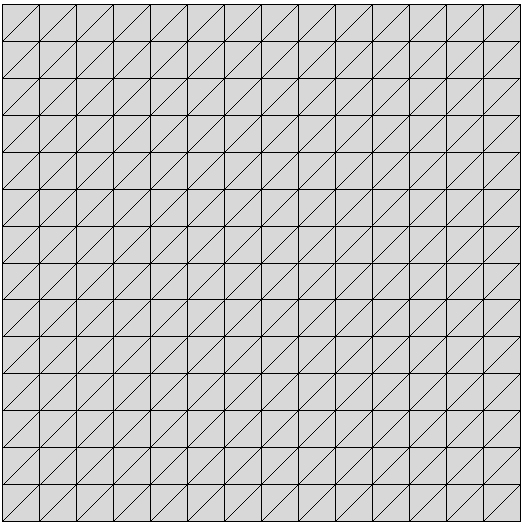
\includegraphics[width=\textwidth]{Chapter2/Graphics/mesh_iso_homo_struct.png}
	\caption{}
    \label{fig:mesh_iso_homo_struct}
  \end{subfigure}
   %------------
   %\hspace{1cm}
   \begin{subfigure}[t]{0.25\textwidth}
    \centering
	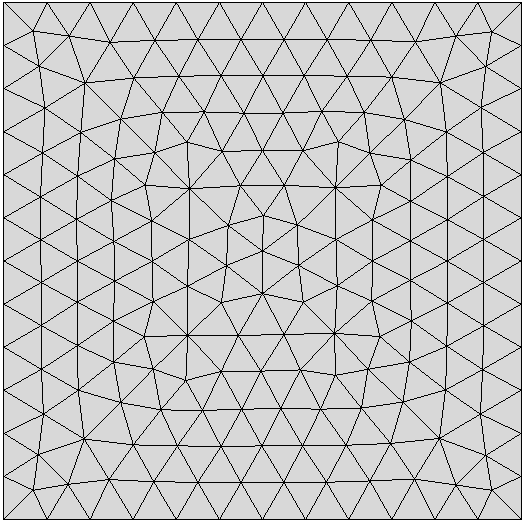
\includegraphics[width=\textwidth]{Chapter2/Graphics/mesh_iso_homo_unstruct.png}
	\caption{}
    \label{fig:mesh_iso_homo_unstruct}
  \end{subfigure}
  %--------
  \vskip\baselineskip
   %------------
  \begin{subfigure}[t]{0.25\textwidth}
    \centering
	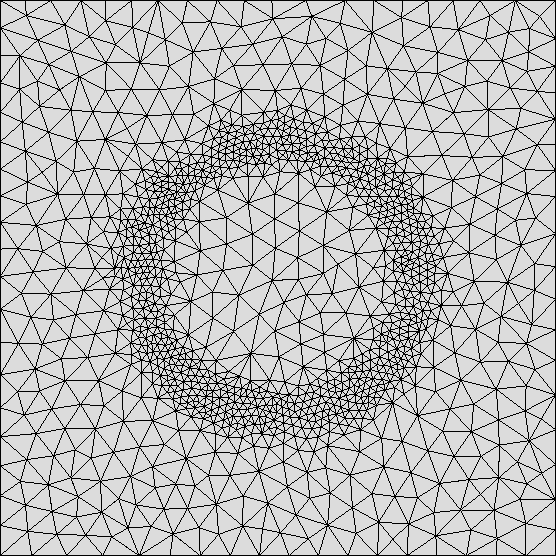
\includegraphics[width=\textwidth]{Chapter2/Graphics/mesh_iso_hetero_unstruct.png}
	\caption{}
    \label{fig:mesh_iso_hetero_unstruct}
  \end{subfigure}
   %------------
   %\hspace{1cm}
   \begin{subfigure}[t]{0.25\textwidth}
    \centering
	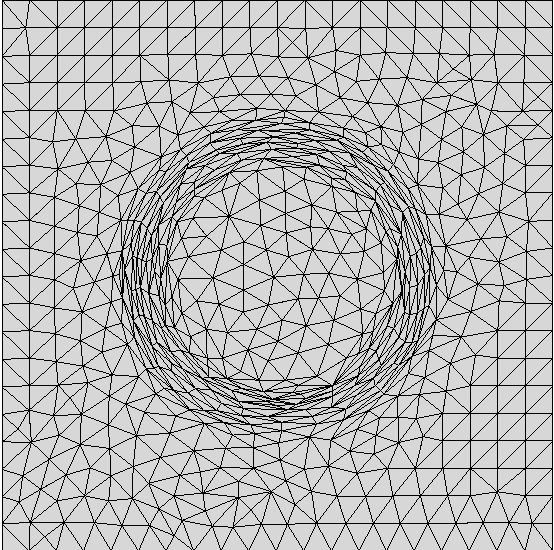
\includegraphics[width=\textwidth]{Chapter2/Graphics/mesh_aniso_hetero_unstruct.png}
	\caption{}
    \label{fig:mesh_aniso_hetero_unstruct}
  \end{subfigure}
  %-------- 
\caption{Alternatives for initial finite element grid generation: (a) structured homogeneous, (b) unstructured homogeneous isotropic,
(c) unstructured heterogeneous isotropic and (d) unstructured heterogeneous anisotropic meshes.} 
\label{fig:premeshing_options}
\end{figure}
%-----------------

Since mesh adaptation involves advanced mathematical notions, readers interested 
in the basics are referred to the following references:
\citep{coupez_grandes_1991,coupez_generation_2000,gruau_3d_2005,jannoun_space-time_2014}.

In this study, we show and compare different remeshing methods relevant to macrosegregation prediction, and based on previous work
done at CEMEF. These techniques rely on metric tensors, and some of them belong to
\emph{a posteriori} error estimators category. A metric or a metric tensor $\mathcal{M}$, 
also known as \emph{Riemannian} metric, is a positive symmetric definite matrix that relates 
to an element's size in $\mathbb{R}^3$ via:
%------
\begin{align}
\label{eq:metric}
& \mathcal{M} = 
\begin{pmatrix}
M_{11} & M_{12} & M_{13} \\
M_{12} & M_{22} & M_{23} \\
M_{13} & M_{23} & M_{33}
\end{pmatrix}
=
\mathcal{R} 
\begin{pmatrix}
1/{h_x^2} & 0 & 0 \\
0 & 1/{h_y^2} & 0 \\
0 & 0 & 1/{h_z^2}
\end{pmatrix}
\mathcal{R}^T
\end{align}
%------------ 
where $\mathcal{R}$ is a rotation matrix and $h_x$, $h_y$ and $h_z$ are the respective 
dilatation scalars defined by the metric in the $\brac{x,y,z}$ space, describing
a three-dimensional anisotropy.
The metric information is then passed to a mesh generation tool, called \emph{MTC},
which is based on an iterative procedure of local topology optimisations. We focus hereafter
on two adaptive remeshing techniques, \emph{Remesh2} and \emph{Remesh4}, then discuss the functional details and show some examples.
Please note that these names represent only a short notation to simplify metionning the corresponding methods easily in the text.

% *********************************************************
\subsection{\emph{Remesh2}: domains boundary remeshing} \label{sec:remesh2_params}
% *********************************************************

\emph{Remesh2} is an explicit \emph{h}-adaptation method to compute an anisotropic metric around the zero surface of a distance function, which defines the boundary between two domains.
The idea is, as mentioned previously, to reduce the elements cost in the tangential directions to level set by
stretching the elements, leaving small element lengths in the normal direction, where the level set gradient is the greatest.
This method is not based on error estimators, but rather on user input to choose the mesh size in
normal and tangential directions to the interface, as well as the mesh size in each of the domains separated by the level set, as shown in \cref{fig:remesh2}.
For more details about this method, the reader is referred to \citep{bernacki_development_2007,resk_adaptive_2009,hitti_direct_2011}.
This remeshing technique relies on the paramater input defined in \cref{table:remesh2_params}.



%--------------------------------
\begin{table}[htbp]
\centering
\caption{Summary of the mesh parameters in order to perform adaptive remeshing based on \emph{Remesh2} technique.}
\label{table:remesh2_params}
{\tabulinesep=1.0mm \begin{tabu}{ll}
\tabucline[1pt]{-}
\textbf{Mesh parameter} & \textbf{Significance} \\\tabucline[1pt]{-}
%-----------------------------
$\varepsilon $			&	level set mixing thickness			\\
$h_{\vec{n}}$ 			&	mesh size in the normal direction to the level set		\\ 
$h_{\vec{\tau}}$ 		&	mesh size in the tangential directions of the level set	\\ 
$h_M$  					&	mesh size in the metal 	\\
$h_A$  					&	mesh size in the air  		\\
Number of nodes 		&   resulting number of nodes after remeshing is done \\
Number of elements 		&   resulting number of elements after remeshing is done  \\\tabucline[1pt]{-}
%-----------------------------
\end{tabu}}
\end{table}
%--------------------------------

%----------------------
\begin{figureth}
% textwidth 
{0.75}
%path 
{Chapter2/Graphics/remesh2.png}
% caption
{(a) Multiple level sets used to delimit the grains of an equiaxial polycrystal with (b) a zoom on the anisotropic mesh elements describing the grain boundaries \citep{hitti_direct_2011}. }
% label
\label{fig:remesh2}
\end{figureth}

%-----------------------------------
% The following parameters are used as input data to determine the final nodal metric field:
% %------------------------------------
% \begin{tabbing}
% \hspace{1cm}\=\kill
% $h_{\vec{n}}$ \> mesh size in the normal direction of the level set\\ 
% $h_{\vec{\tau}}$ \> mesh size in the tangential directions of the level set\\ 
% $h_M$ \>  mesh size in the metal \\
% $h_A$ \>  mesh size in the air  \\
% $\levelset$ \> distance function (level set) \\
% $\varepsilon$ \>  level set mixing thickness \\
% $\vec{V}$ \> arbitrary vector
% \end{tabbing} 
% %------------------------------------
% \begin{algorithm}[H]
%  \KwData{$\vec{n}\quad h_M \quad h_A \quad h_{\vec{n}} \quad h_{\vec{\tau}} \quad \levelset$ }
%  \KwResult{$\mathcal{M}_2$ }
%  Initialise node index: $j=0$\;
%  \While{$j \leq j_\text{end}$}{
%   \eIf{$\levelset_j < \varepsilon$}{
%     Compute normal direction to level set: $\vec{n} ={\nabvec \levelset }/{\norm{\nabvec \levelset }}$\;
%     Compute the first tangential direction: $\vec{\tau_1} = \vec{V} - \brac{\vec{V} \cdot \vec{n}}\cdot \vec{n}$\;
%     Deduce the second tangential direction: $\vec{\tau_2} = \vec{n} \wedge \vec{\tau_1}$\;
%     Compute rotation matrix and its transpose: $\mathcal{R}_j$ and $\mathcal{R}_j^{-1}$\;
%     Deduce P1 metric at node $j$: $\brac{\mathcal{M}_2}_j = \mathcal{R}_j \Lambda \mathcal{R}_j^{-1}$
%    }{
%    go back to the beginning of current section\;
%   	}
%   Increment $j$ \;	
%   }  
%  \caption{\emph{Remesh2} metric construction}
% \end{algorithm}

% ******************************************************
\subsection{\emph{Remesh4}: Multi-criteria remeshing}   \label{sec:remesh4_params}
% ******************************************************

It is essentially an \emph{a posteriori} error estimator. The method consists of estimating the interpolation error for
one or more nodal fields, then using a statistical concept, the so-called \emph{length distribution tensor}, a stretching factor
can be determined by solving several constraints like locally minimizing the induced error, limit the number of created nodes to
a specific  threshold, etc. Finally, the stretching factor is directly used to correct the edge lengths, where the latter varies in such a way to minimize the locally induced error down
to a specified error limit, $\varepsilon_\text{er.}$.
For detailed technical information, the reader is referred to these references: \citep{coupez_metric_2011,coupez_edge-based_2013,el_jannoun_space-time_2014}.

This method is readily compatible with multiple scalar or vector input, which results in a final metric accounting
for the steepness of each quantity gradient. In solidification, such a technique is appealing since we often need 
to maintain a sufficiently small mesh size in areas of interest, e.g. narrow mushy zone formation caused by high thermal gradients, areas with composition variations or
areas where fluid convection is a consequence to combined effects of energy-solute variations. \Cref{fig:remesh4} shows an example of mechanically driven flow,
along with the accurate capturing of the interface using highly stretched anisotropic elements, at the edges and in the centre.

This remeshing technique relies on the parameter input defined in \cref{table:remesh4_params}.
Among the parameters, $h_\text{min}$ and $\varepsilon_\text{er.}$ are the most important.
The first one sets the minimum limit for the mesh algorithm to take while topoligically optimising the grid. 
The seconds parameter controls the error, and hence globally the elements shape may vary from highly anisotropic 
shapes (low values of $\varepsilon_\text{er.}$), to isotropic (high values of $\varepsilon_\text{er.}$).
We prefer to limit this parameter by using a reasonable value, between 10 and 500, depending on the case and the final results.


%-----------------
\begin{figure}[H]
\centering
   %------------
  \begin{subfigure}[t]{0.3\textwidth}
    \centering
 	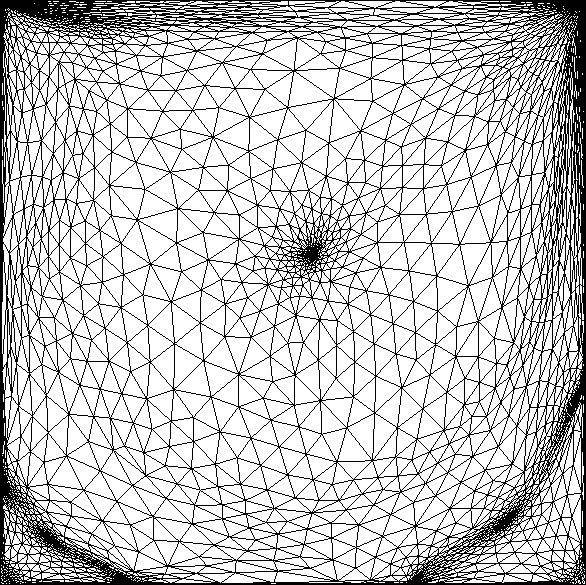
\includegraphics[width=\textwidth]{Chapter2/Graphics/remesh4_1000.png}
	\caption{}
  \end{subfigure}
   %------------
   %\hspace{1cm}
   \begin{subfigure}[t]{0.3\textwidth}
    \centering
	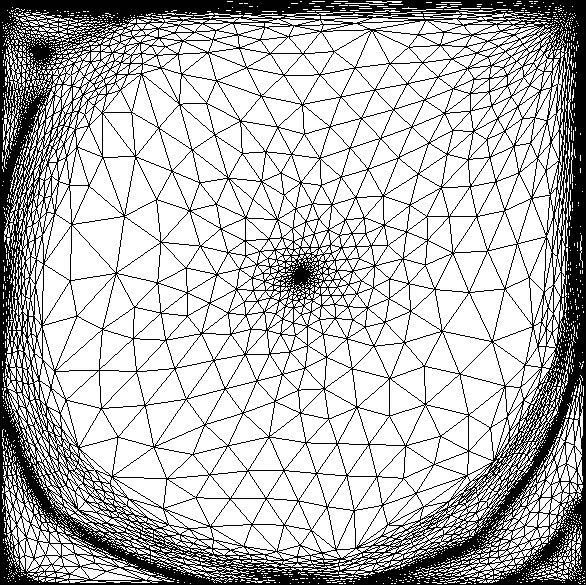
\includegraphics[width=\textwidth]{Chapter2/Graphics/remesh4_10000.png}
	\caption{}
  \end{subfigure}
   %------------
  \begin{subfigure}[t]{0.3\textwidth}
    \centering
	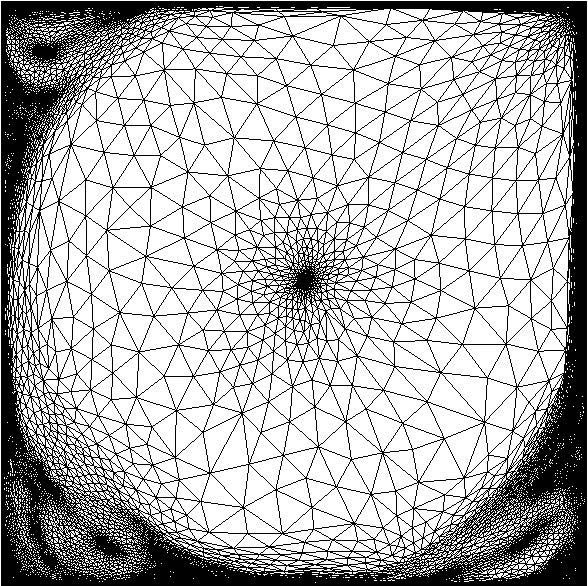
\includegraphics[width=\textwidth]{Chapter2/Graphics/remesh4_100000.png}
	\caption{}
  \end{subfigure}
  %-------- 
\caption{Edge-based anisotropic metric generation applied to a driven flow inside cavity with a Reynolds number of 
(a) \num{1000} (b) \num{10000} and (c) \num{100000} \citep{coupez_edge-based_2013}. } 
\label{fig:remesh4}
\end{figure}
%-----------------

 %--------------------------------
\begin{table}[htbp]
\centering
\caption{Summary of the mesh parameters in order to perform adaptive remeshing based on \emph{Remesh4} technique.}
\label{table:remesh4_params}
{\tabulinesep=1.0mm \begin{tabu}{ll}
\tabucline[1pt]{-}
\textbf{Mesh parameter} & \textbf{Significance} \\\tabucline[1pt]{-}
%-----------------------------
$\varepsilon $			&	level set mixing thickness			\\
$h_\text{min}$			&   minimum mesh size \\
$\varepsilon_\text{er.}$	&  minimum error limit \\
Remeshing criteria 	 	&   physical quantities of interest \\
Number of nodes 		&   resulting number of nodes after remeshing is done \\
Number of elements 		&   imposed number of elements needed for the remesh optimisation  \\\tabucline[1pt]{-}
%-----------------------------
\end{tabu}}
\end{table}
%--------------------------------

% What i concluded from Z-FAST-SMACS cases A and B, where remesh4 was used in two different ways (LS and velocity/100  ,  LS and ConcentrationPosNeg)
% is that for diffuse interface thickness less than 2e-4 m, mass conservation gets all sorts of problems, because of low element resolution 
% around interface while higher resolution at the tips of the transition region


% \section*{To do ?}
% \comment{Interface Remeshing: Importance when using a static level set and more importantly when LS is transported,
% influence of mixing area \emph{thickness} and \emph{resolution} (i.e. nb of nodes with the area),
% Isotropic or anisotropic ? the first is more important to composition calculation while the second
% is more relevant if we mean do thermohydraulics without macrosegregation}



\clearpage
\section*{Résumé chapitre 2}

\begin{otherlanguage}{french}
{\small
Le second chapitre de ce manuscrit présente une revue de la littérature, concernant les aspects de modélisation utilisés dans ce travail.
Au début, on présente quelques approches connues pour modéliser l'effet de la microségrégation sur la variation des fractions de phases ainsi que leurs compositions.
On s'intéresse après à l'approche de prise de moyenne volumique. Celle-ci nous permet de faire des hypothèses sur des petits volumes, qualifiés de \emph{volumes élémentaires représentatifs},
permettant d'établir des relations pour l'ensemble des propriétés des phases. En utilisant ces relations, on présente la première brique numérique de ce travail: les équations
de conservation de masse, énergie, solutés et quantité de mouvement dans un contexte de solidification à volume constant, donc sans retrait. Le modèle est complété par une hypothèse de 
solide fixe et rigide qui permet de négliger tout movement des phases solides, et donc la thermomécanique de ces phases n'est pas traitée.
Dans la suite du chapitre, on présente les descriptions eulérienne et lagrangienne caractérisant l'écoulement de la phase liquide. 
Cela s'avère nécessaire dans un contexte de solidification avec changement de volume, où l'interface entre le métal et le milieu ambiant change au cours de la transformation.
Par conséquent, le choix de la méthode level set pour le suivi de cette interface est expliqué. On présente aussi des méthodes numériques pour prendre en compte le mouvement
de l'interface suivie par la méthode level set, dans le contexte eulérien. Finalement, deux méthodes de remaillage adaptatif, utilisé pour l'ensemble des calculs faits pendant la thèse,
sont présentés et expliqués, tout en montrant leurs avantages et leurs inconvénients.
}
\end{otherlanguage} % resume francais